\documentclass[11pt]{article}

% ── Packages ──────────────────────────────────────────────────────────────────
\usepackage[margin=1in]{geometry}
\usepackage{graphicx}
\usepackage{booktabs}
\usepackage{amsmath}
\usepackage{amssymb}
\usepackage{hyperref}
\usepackage{xcolor}
\usepackage{microtype}
\usepackage[numbers,sort&compress]{natbib}
\usepackage{subcaption}

\hypersetup{
  colorlinks=true,
  linkcolor=blue!60!black,
  citecolor=blue!60!black,
  urlcolor=blue!60!black,
}

\graphicspath{{figures/}}

% ── Title ─────────────────────────────────────────────────────────────────────
\title{Noesis: Selective Memory Injection for\\Cross-Tool AI Conversation Consistency}

\author{%
  Anonymous\\
  \texttt{https://github.com/AngryKiwiWithLegs/Noesis}
}
\date{August 2026}

\begin{document}
\maketitle

% ══════════════════════════════════════════════════════════════════════════════
\begin{abstract}
Users converse with multiple AI assistants daily, yet each tool's memory is
isolated: a stance expressed in one tool is unknown to the others, and each
conversation starts from scratch. Existing approaches either store flat facts
without a notion of confidence, or inject all retrieved context regardless of
relevance, causing token costs to explode with memory size. We present
\textbf{Noesis}, a local-first memory layer that (1) extracts typed
\emph{thoughts} from conversations across tools into a shared per-user store,
(2) gates injection behind a confidence lifecycle in which thoughts mature from
\emph{tentative} to \emph{settled} based on repetition, assertion strength,
cross-tool corroboration, and contradiction signals, and (3) caps injected
context with a token budget. Across three models (Gemini Flash, gemma3:4b,
qwen2.5:3b) on 110 paired questions each, memory injection raises answer
accuracy from 41.8\% to 85.5\%, 34.5\% to 82.7\%, and 37.3\% to 62.7\%
respectively (all $p<0.001$, McNemar's test). At 500 stored memories, Noesis
injects 35$\times$ fewer tokens than a naive RAG baseline while maintaining
rank-1 retrieval (MRR 0.90 vs.\ 0.002). Cross-tool retrieval reaches 50\%
where per-tool isolation is structurally bound to 0\%. We release the system,
experiment harness, and all raw results.
\end{abstract}

% ══════════════════════════════════════════════════════════════════════════════
\section{Introduction}
\label{sec:intro}

Heavy users of AI assistants switch between ChatGPT, Claude, Gemini, and local
models throughout the day. Each tool maintains its own isolated memory: a
database preference carefully explained to Claude must be re-explained to
GPT; a design decision reached with Gemini is invisible to Claude. The
reasoning a user performs across tools---their positions, preferences, and
open questions---evaporates at every tool boundary.

Two families of systems address parts of this problem, each with a critical
gap. \emph{Fact stores} such as Mem0~\citep{mem0} persist extracted facts but
treat all memories equally: a firmly held professional identity and a
passing mention of a tool have the same standing, and there is no mechanism
for a memory to earn trust over time. \emph{Retrieval-augmented generation}
(RAG)~\citep{lewis2020rag} retrieves relevant context for each query, but
naive variants inject everything retrieved; as personal memory grows into
the hundreds of items, injected context grows linearly, burying the relevant
signal and inflating cost (we measure 7{,}192 tokens at $n{=}500$).

Noesis is built on a different premise: \emph{what} gets injected matters as
much as \emph{whether} anything is injected. Thoughts should earn their way
into the context the way beliefs earn their way into a mind---through
repetition, consistency, and survival against contradiction.

This paper makes the following contributions:

\begin{enumerate}
  \item \textbf{A confidence lifecycle for conversational memory}
  (\S\ref{sec:system}). Thoughts are typed (identity, preference, position,
  question, synthesis, event, contradiction) and mature
  tentative$\to$provisional$\to$settled via a four-signal scorer, with
  type-specific time decay and cluster-aware supersession that reduced
  stale-stance leakage from 93\% to 7\% (\S\ref{sec:supersession}).
  \item \textbf{Budget-capped selective injection that scales}
  (\S\ref{sec:scale}). At 500 memories Noesis injects $\sim$207 tokens
  (35$\times$ fewer than naive RAG) while holding MRR at 0.90; naive RAG's
  MRR collapses to 0.002 as targets are buried (\S\ref{sec:scale}).
  \item \textbf{Quantified cross-tool memory sharing} (\S\ref{sec:crosstool}).
  With a shared per-user store, cross-tool retrieval reaches 50\% (37\% on
  strictly cross-tool queries) versus \textbf{0\%} for per-tool
  isolation---a gap that is architecturally impossible for isolated systems
  to close.
  \item \textbf{A replicated A/B result across model tiers}
  (\S\ref{sec:ab}). On identical $n{=}110$ question sets, memory injection
  significantly improves answer accuracy for a cloud model (Gemini Flash,
  $+43.6$pp), a mid-tier local model (gemma3:4b, $+48.2$pp), and a small
  local model (qwen2.5:3b, $+25.5$pp); all $p<0.001$.
\end{enumerate}

The system is local-first: embeddings and retrieval run on-device
(sqlite-vec + all-MiniLM-L6-v2), and only optional LLM-based extraction calls
a cloud API. All code, the experiment harness, raw results, and a
verification script that recomputes every reported number from raw JSON are
released.\footnote{\url{https://github.com/AngryKiwiWithLegs/Noesis}}

\begin{figure}[t]
  \centering
  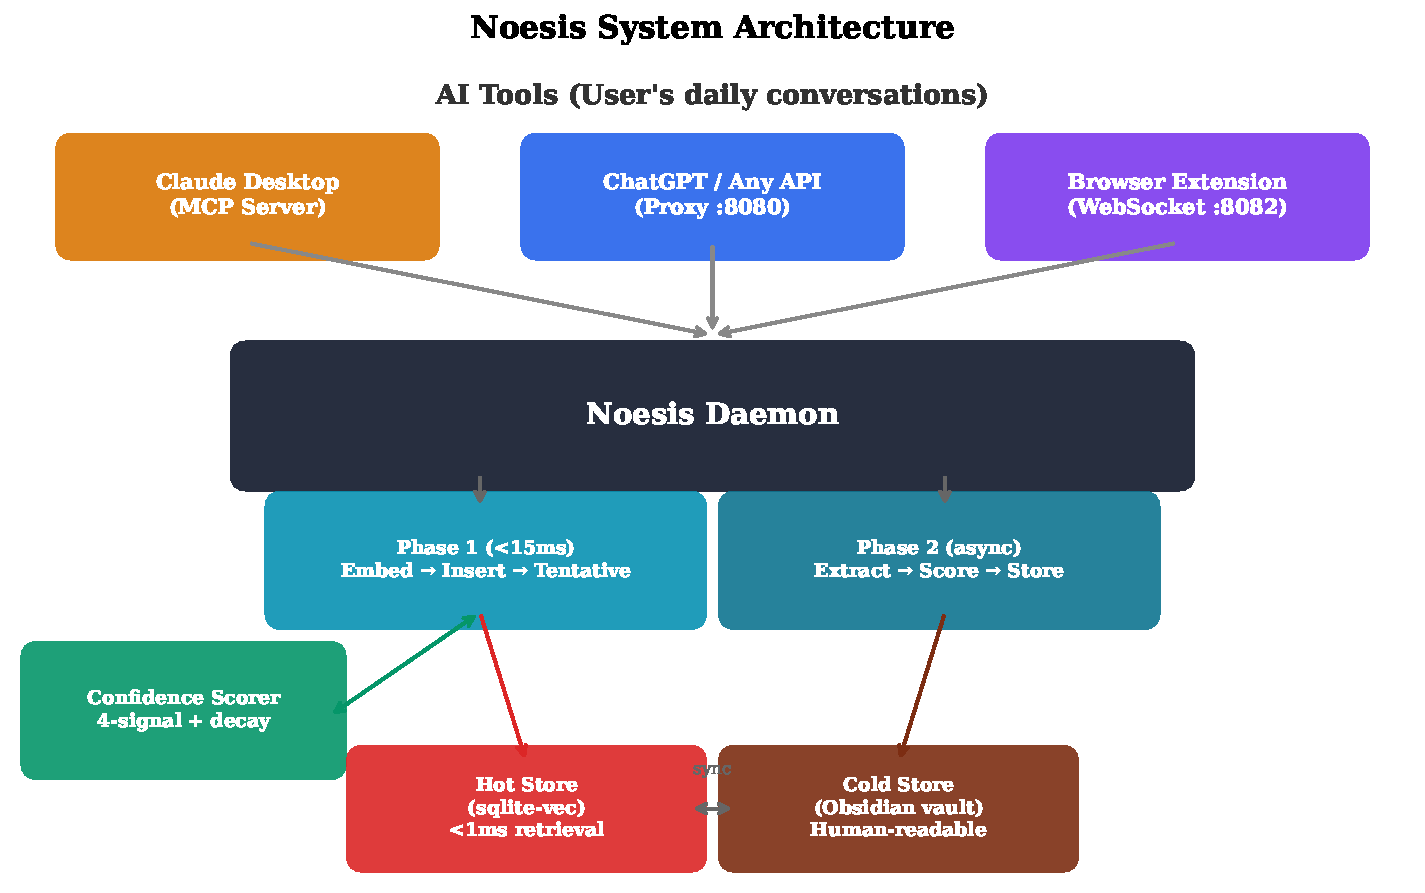
\includegraphics[width=0.95\linewidth]{fig1_architecture.pdf}
  \caption{Noesis system architecture. Any OpenAI-compatible tool routes
  through the local proxy; Phase 1 stores the utterance synchronously
  ($<$15\,ms) and Phase 2 asynchronously extracts, scores, and links the
  thought. Hot store (sqlite-vec) serves retrieval; cold store (Obsidian
  vault) keeps memory human-readable and editable.}
  \label{fig:architecture}
\end{figure}

% ══════════════════════════════════════════════════════════════════════════════
\section{Related Work}
\label{sec:related}

\paragraph{Memory for LLM agents.}
MemGPT~\citep{memgpt} treats the LLM as an operating system paging memory
between contexts; Letta extends this with archival storage. Mem0~\citep{mem0}
extracts and updates atomic facts with an LLM pipeline, reporting gains over
full-history baselines. These systems store \emph{facts}; none models the
\emph{confidence} of a memory over time, and none addresses multiple
front-end tools sharing one user's memory. Noesis differs in (a) its
lifecycle, where injection rights are earned, and (b) its tool-agnostic
proxy architecture, which makes any OpenAI-compatible client a first-class
participant.

\paragraph{Retrieval-augmented generation.}
RAG~\citep{lewis2020rag} and successors retrieve per-query context.
Self-RAG~\citep{selfrag} and FLARE~\citep{flare} improve retrieval quality
or adaptivity, but address corpus QA, not a user's evolving personal memory.
Our scale experiment (\S\ref{sec:scale}) shows why naive inject-everything
retrieval fails for personal memory: cost grows linearly and ranking
collapses. Noesis pairs hybrid retrieval (BM25 + vector + RRF, with
time-decay weighting) with a hard token budget and a confidence gate.

\paragraph{Personalization.}
PALR~\citep{palr} and related work personalize outputs from user interaction
history, typically for recommendation-style tasks. Chat-tool vendor memory
features (e.g., ChatGPT memory) are per-product and closed. Noesis's
cross-tool experiment (\S\ref{sec:crosstool}) demonstrates a structural
advantage of user-scoped rather than tool-scoped memory.

\paragraph{Visualization of embedding spaces.}
t-SNE~\citep{tsne} and UMAP~\citep{umap} project high-dimensional
embeddings for inspection; force-directed layouts~\citep{forcedirected}
model attraction/repulsion in 2D. Our star map (\S\ref{sec:viz}) extends
force-directed layout to 3D with a time-spring axis so that semantic
clusters remain volumetric while recency reads as height.

% ══════════════════════════════════════════════════════════════════════════════
\section{System Design}
\label{sec:system}

Noesis sits between AI tools and model providers (Figure~\ref{fig:architecture}).
Tools point at a local OpenAI-compatible proxy; the proxy injects memory
into the system prompt, forwards the request to the configured provider
(cloud or local), and captures the conversation for memory formation.

\subsection{Thought taxonomy and two-phase capture}
\label{sec:taxonomy}

Conversational memory is typed into seven categories with distinct
persistence semantics (Table~\ref{tab:thought_types}). An \emph{identity}
thought (``I am a backend engineer'') should outlive an \emph{event}
(``I tried Bun yesterday''), and the taxonomy encodes this as type-specific
half-lives.

Capture is two-phase. \emph{Phase 1} is synchronous and bounded ($<$15\,ms):
embed, deduplicate by hash, insert as \emph{tentative}. The conversation
never blocks on memory. \emph{Phase 2} is asynchronous: an extractor (a
small cloud LLM, or a deterministic fallback) classifies the thought; a
confidence scorer updates its status; a supersession check retires
contradicted predecessors; the cold store (Markdown + YAML frontmatter in an
Obsidian vault) is updated for human readability and editability.

\begin{table}[t]
  \centering
  \caption{Thought taxonomy with type-specific half-lives and injection priority.}
  \label{tab:thought_types}
  \begin{tabular}{llcc}
    \toprule
    \textbf{Type} & \textbf{Definition} & \textbf{Half-life (days)} & \textbf{Priority} \\
    \midrule
    identity      & Who the user is                 & $\infty$ & highest (always) \\
    preference    & Explicit preference             & 90       & high \\
    position      & Stance on a topic               & 90       & high \\
    question      & Open question under exploration & 30       & medium \\
    synthesis     & Insight from merged ideas       & 180      & medium \\
    event         & Happened / decided              & 7        & low (recent) \\
    contradiction & Self-contradictory judgment     & $\infty$ & flagged \\
    \bottomrule
  \end{tabular}
\end{table}

\subsection{Confidence lifecycle}
\label{sec:lifecycle}

Every thought begins \emph{tentative}: stored, but never injected and
invisible to retrieval---the ``capture threshold low, injection threshold
high'' principle. Four signals promote a thought: \emph{repetition} (the
same stance recurs across sessions), \emph{assertion strength} (``I've
decided'' outranks ``maybe''), \emph{cross-tool consistency} (distinct
phrasings of a stance from different tools), and \emph{absence of
contradiction}. \emph{Provisional} thoughts inject when topic-relevant;
\emph{settled} thoughts always inject. Confidence evolves incrementally:
reinforcement $+0.10\,(1-C)$, conflict $-0.20$, and time decay
$C \leftarrow C\, e^{-0.693\,\Delta t / t_{1/2}}$ with $t_{1/2}$ set by type
(Table~\ref{tab:thought_types}).

\subsection{Cluster-aware supersession}
\label{sec:supersession}

When a user changes their mind (``I moved from MySQL to PostgreSQL''), the
old stance should retire. Embedding similarity is the wrong signal here:
contradictory stances mention different entities and therefore have
\emph{low} similarity. Noesis detects mind-changes by requiring jointly (1)
a replacement verb (``switched to'', ``migrated to'', \ldots, EN+ZH), (2)
the same domain via a keyword map (both stances are about \emph{databases}),
(3) stance-like type, and (4) injectable status of the new thought.
Matched predecessors are marked \emph{superseded}---excluded by every
retrieval path---and linked via \texttt{superseded\_by}. In our evaluation
this reduced stale-stance leakage from 93\% to 7\%
(Table~\ref{tab:supersession}).

\begin{table}[t]
  \centering
  \caption{Supersession fix: stale-stance leakage before/after ($n{=}30$ scenarios).}
  \label{tab:supersession}
  \begin{tabular}{lccc}
    \toprule
    \textbf{Metric} & \textbf{Before} & \textbf{After} & \textbf{$\Delta$} \\
    \midrule
    Old stance leaked into context & 28/30 (93\%) & 2/30 (7\%)  & $-86$pp \\
    New stance surfaced            & 12/30 (40\%) & 28/30 (93\%) & $+53$pp \\
    Ideal (new shown, old retired) & 1/30 (3\%)   & 26/30 (87\%) & $+84$pp \\
    \bottomrule
  \end{tabular}
\end{table}

\subsection{Selective retrieval and injection}
\label{sec:retrieval}

At query time, three channels run in parallel (Figure~\ref{fig:pipeline}):
BM25 for exact terms, dense retrieval for paraphrase, and two lightweight
signals (recency, core-facts). Channels fuse via reciprocal-rank fusion with
time-decay weighting. A confidence gate drops everything below
\emph{provisional}, and a hard token budget (1{,}200 tokens) truncates the
remainder. The result is injected into the system prompt as compact
structured lines.

\begin{figure}[t]
  \centering
  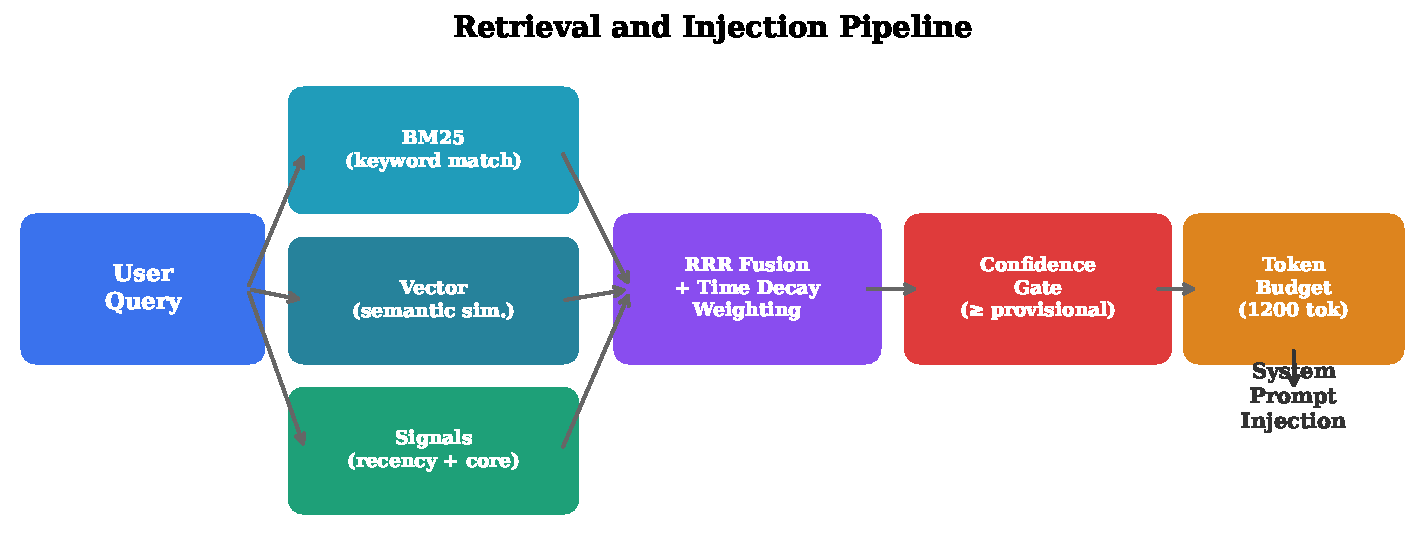
\includegraphics[width=\linewidth]{fig2_pipeline.pdf}
  \caption{Retrieval and injection pipeline. Three channels fuse via RRF;
  a confidence gate removes non-injectable thoughts; a token budget caps
  injected context.}
  \label{fig:pipeline}
\end{figure}

% ══════════════════════════════════════════════════════════════════════════════
\section{Evaluation Setup}
\label{sec:setup}

We evaluate four research questions:

\begin{itemize}
  \item \textbf{RQ1}: Does memory injection improve answer accuracy?
        (A/B, end-to-end, \S\ref{sec:ab})
  \item \textbf{RQ2}: Which components contribute? (ablation,
        retrieval-layer, \S\ref{sec:ablation})
  \item \textbf{RQ3}: How do cost and ranking scale with memory size?
        (\S\ref{sec:scale})
  \item \textbf{RQ4}: Does cross-tool sharing work? (\S\ref{sec:crosstool})
\end{itemize}

\paragraph{Models.} Gemini Flash (cloud), gemma3:4b and qwen2.5:3b (local
via Ollama), spanning capability tiers.

\paragraph{A/B design.} 30 synthetic English user profiles, each with 5
build statements (identity/preference/position/event/fact) followed by 5
test questions whose expected keyword is known from the build statements.
For each question the model answers twice: \emph{with memory} (via the
Noesis proxy, which injects context) and \emph{without memory} (direct to
the provider). All models are evaluated on the identical first
$110$ questions (22 profiles). Scoring is objective keyword-hit; paired
outcomes are tested with McNemar's $\chi^2$.

\paragraph{Retrieval-layer experiments.} Ablation, scale, and cross-tool
experiments run against the real pipeline without LLM calls, measuring
Recall@5, MRR, Precision@5, tentative leakage, and injected tokens.

\paragraph{Reproducibility.} Every number in this paper is recomputed from
raw JSON by a released verification script.

% ══════════════════════════════════════════════════════════════════════════════
\section{Results}
\label{sec:results}

\subsection{RQ1: Memory injection improves accuracy across model tiers}
\label{sec:ab}

\begin{table}[t]
  \centering
  \caption{A/B results on identical $n{=}110$ questions. All $p<0.001$
  (McNemar, df$=$1).}
  \label{tab:ab_results}
  \begin{tabular}{lccccc}
    \toprule
    \textbf{Model} & $n$ & \textbf{With} & \textbf{Without} & $\Delta$pp & $\chi^2$ \\
    \midrule
    Gemini Flash & 110 & 85.5\% & 41.8\% & \textbf{+43.6} & 42.48 \\
    gemma3:4b    & 110 & 82.7\% & 34.5\% & \textbf{+48.2} & 51.02 \\
    qwen2.5:3b   & 110 & 62.7\% & 37.3\% & \textbf{+25.5} & 16.57 \\
    \bottomrule
  \end{tabular}
\end{table}

\begin{figure}[t]
  \centering
  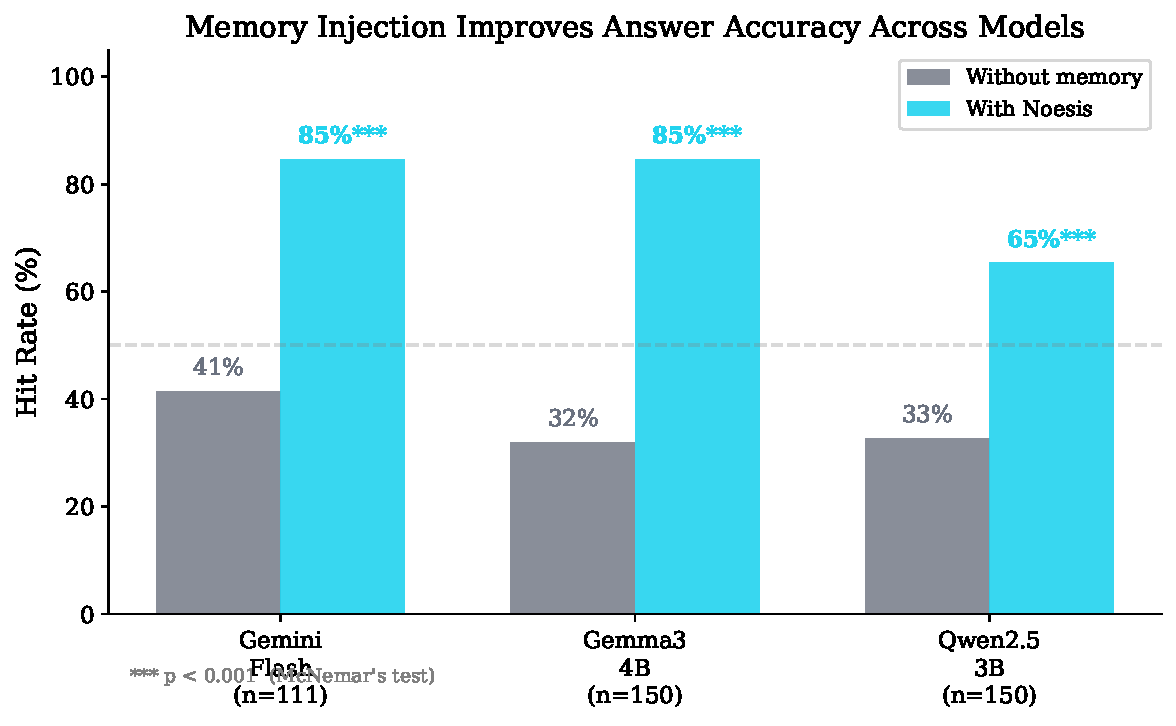
\includegraphics[width=0.9\linewidth]{fig3_ab_comparison.pdf}
  \caption{A/B accuracy across models ($n{=}110$ each). All improvements
  significant at $p<0.001$.}
  \label{fig:ab}
\end{figure}

Table~\ref{tab:ab_results} and Figure~\ref{fig:ab} show the headline
result. Three findings stand out. First, \emph{injection helps everywhere}:
all three models improve significantly, and memory \emph{hurt} in only 10 of
330 paired answers (3.0\%). Second, \emph{memory levels the field between
local and cloud}: with injection, gemma3:4b (4B parameters, local) reaches
82.7\%, nearly matching Gemini Flash's 85.5\%, while its no-memory baseline
(34.5\%) trails Gemini's 41.8\%. Third, \emph{small models are
comprehension-capped}: qwen2.5:3b receives the same injected context but
reaches only 62.7\%; inspection shows the memory was present in-prompt and
the model failed to use it---a model-capability ceiling, not a retrieval
failure.

\subsection{RQ2: Semantic retrieval is the engine; gating is the moat}
\label{sec:ablation}

\begin{table}[t]
  \centering
  \caption{Ablation and baselines (50 queries, retrieval-layer).}
  \label{tab:ablation}
  \begin{tabular}{lcccc}
    \toprule
    \textbf{Config} & \textbf{Recall@5} & \textbf{MRR} & \textbf{Prec@5} & \textbf{Leak} \\
    \midrule
    \textbf{Noesis (full)}   & \textbf{100\%} & \textbf{1.000} & \textbf{96\%} & \textbf{10} \\
    w/o core-fact signal     & 100\% & 1.000 & 96\% & 10 \\
    w/o recency signal       & 100\% & 1.000 & 96\% & 10 \\
    w/o confidence gating    & 100\% & 1.000 & 88\% & \textbf{29} \\
    w/o semantic retrieval   & 49\%  & 0.160 & 100\% & 0 \\
    \midrule
    Naive RAG                & 100\% & 1.000 & 88\% & 29 \\
    Recent-window            & 22\%  & 0.099 & 100\% & 0 \\
    Random                   & 45\%  & 0.206 & 94\% & 15 \\
    \bottomrule
  \end{tabular}
\end{table}

Removing semantic retrieval collapses recall (100\%$\to$49\%), confirming it
as the engine (Table~\ref{tab:ablation}). Removing the confidence gate
leaves recall intact but leaks 29 tentative thoughts versus 10---gating is
what keeps \emph{unverified} material out of the prompt. Core-fact and
recency signals show no measurable effect in this query-driven suite; their
value emerges on identity-relevant but topically unrelated queries, which
this suite undersamples (an honest gap).

\subsection{RQ3: Cost stays flat while baselines explode}
\label{sec:scale}

\begin{figure}[t]
  \centering
  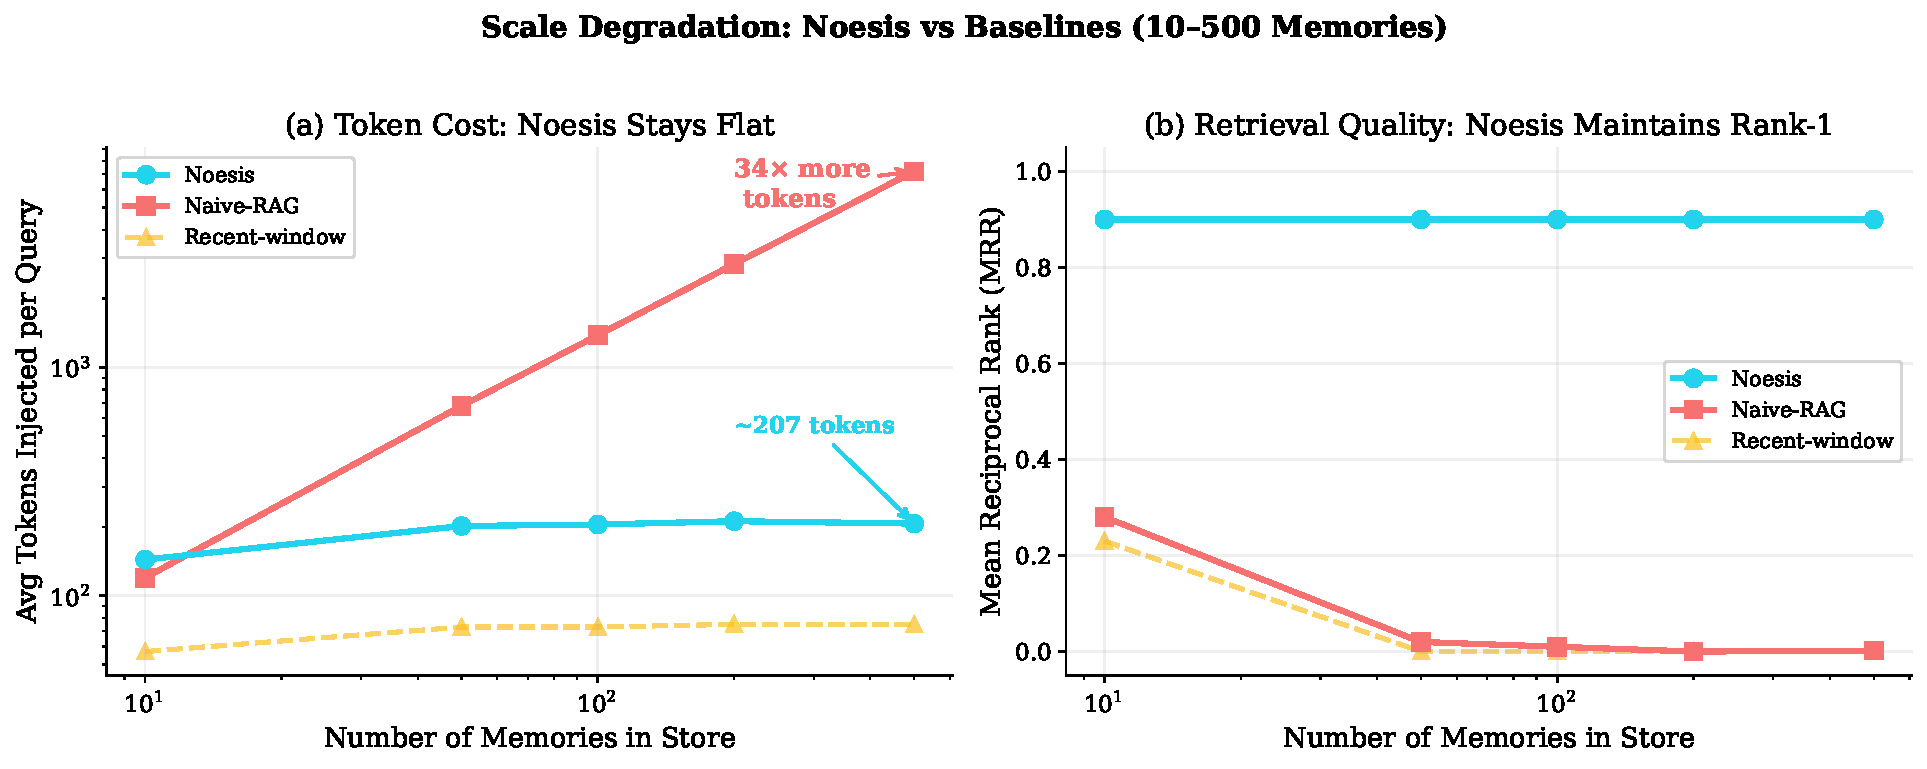
\includegraphics[width=\linewidth]{fig4_scale_degradation.pdf}
  \caption{Scale behavior from 10 to 500 stored memories. (a) Noesis's
  injected tokens stay flat ($\sim$207) while naive RAG grows to 7{,}192
  (35$\times$). (b) Noesis holds MRR at 0.90; naive RAG collapses to 0.002
  as targets are buried; recent-window loses recall entirely past $n{=}10$.}
  \label{fig:scale}
\end{figure}

Figure~\ref{fig:scale} sweeps memory size from 10 to 500 with 10 known
targets embedded among fillers. Noesis's injected cost is flat
(144$\to$207 tokens) because the budget caps it by construction, and MRR
holds at 0.90---the target sits at rank 1. Naive RAG keeps recall only by
injecting everything: 7{,}192 tokens at $n{=}500$, with the target buried
near rank 500 (MRR 0.002). Recent-window recall collapses to 0\% beyond
$n{=}10$: the window forgets everything older. The methodological takeaway:
\emph{recall alone is misleading}; rank and token cost must be reported
together.

\subsection{RQ4: Cross-tool sharing vs.\ structural isolation}
\label{sec:crosstool}

\begin{figure}[t]
  \centering
  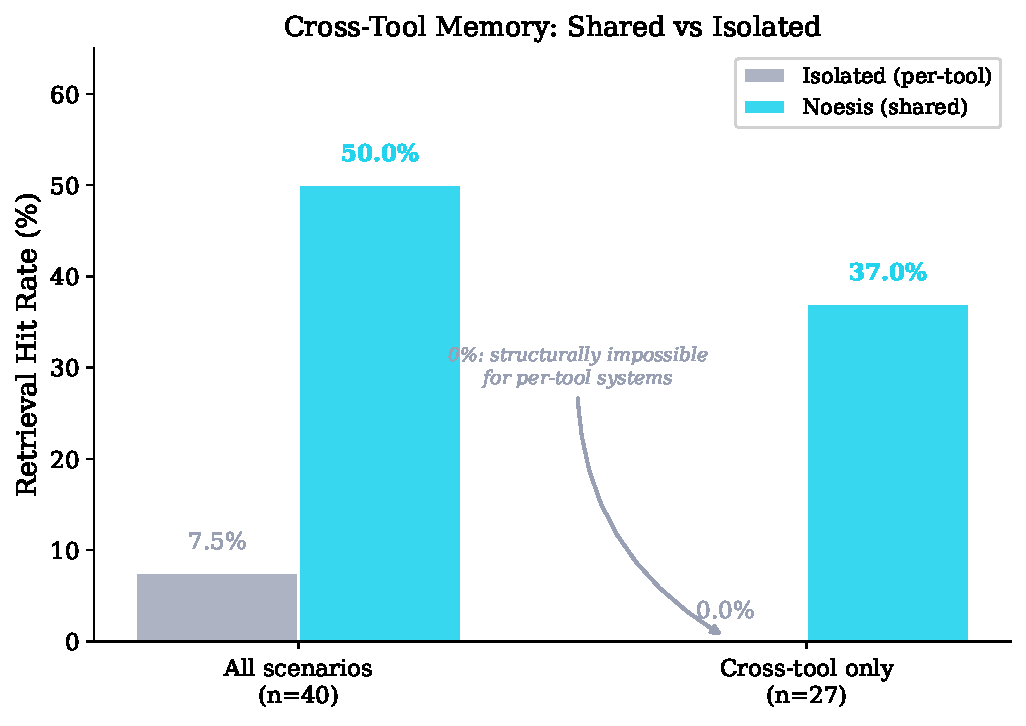
\includegraphics[width=0.85\linewidth]{fig6_cross_tool.pdf}
  \caption{Cross-tool retrieval. Isolated per-tool memory scores 0\% on
  strictly cross-tool queries by construction.}
  \label{fig:crosstool}
\end{figure}

In 40 scenarios a stance stated under tool A is queried under tool B
(Figure~\ref{fig:crosstool}). Noesis retrieves 50\% overall and 37\% on
strictly cross-tool queries; the isolated baseline retrieves \textbf{0\%}
on the latter---not because it ranks poorly, but because the memory is not
in its partition. This is the structural argument: per-tool memory systems
cannot share by design, and no amount of per-tool tuning closes the gap.
Noesis's misses trace to retrieval precision (the memory exists but ranks
below top-$k$), not to sharing.

% ══════════════════════════════════════════════════════════════════════════════
\section{The Star Map Visualization}
\label{sec:viz}

\begin{figure}[t]
  \centering
  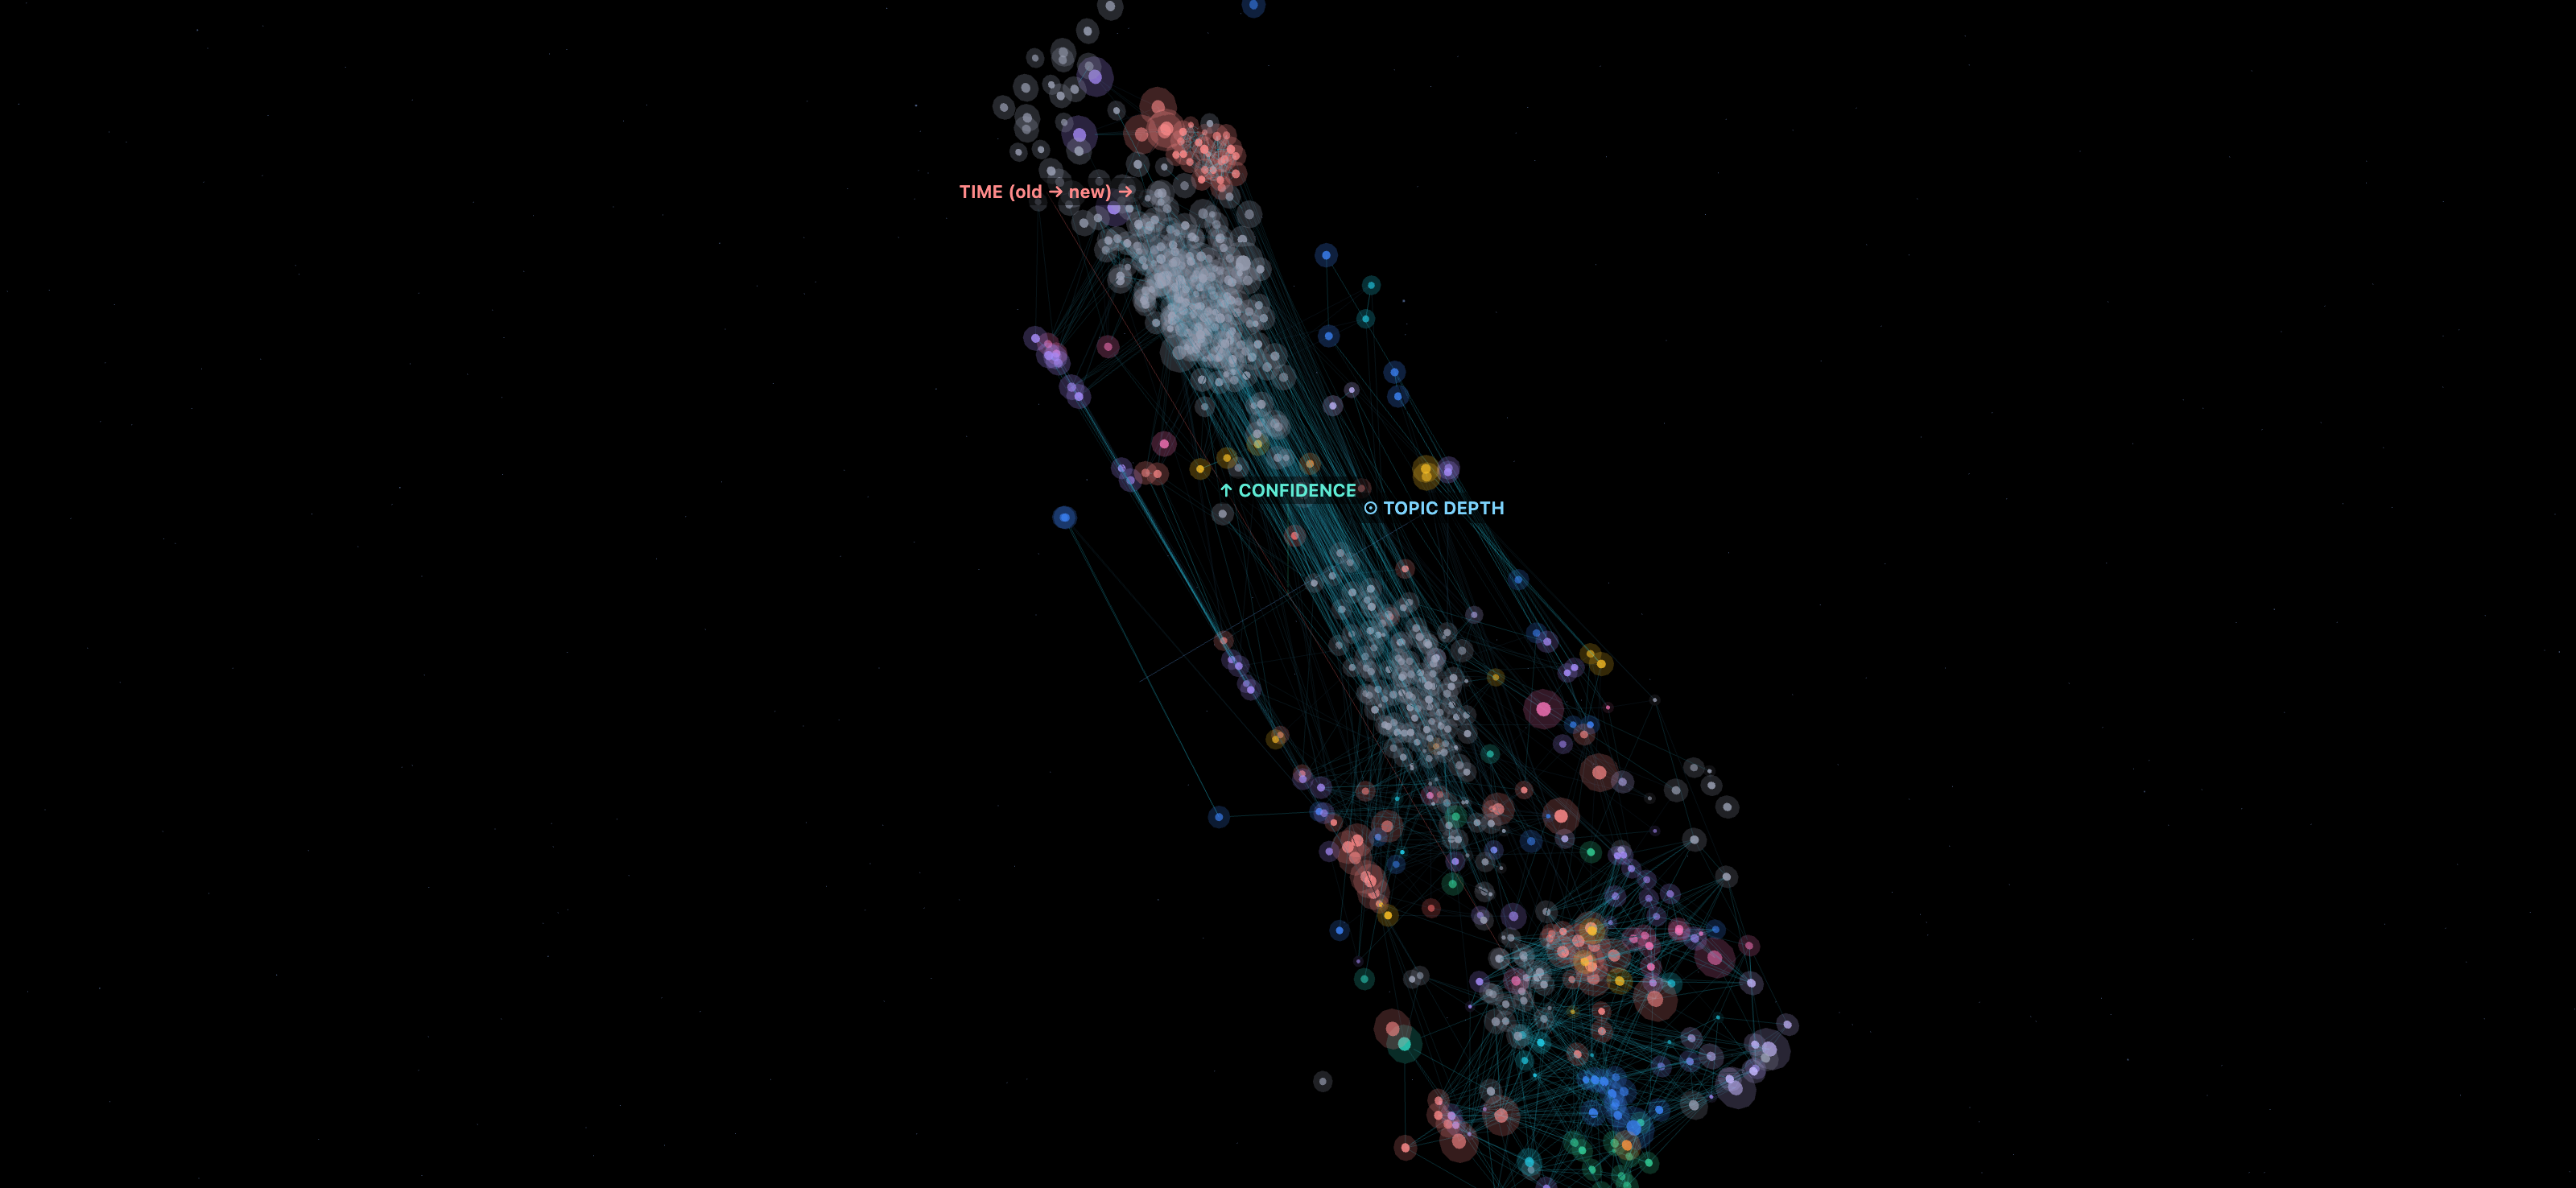
\includegraphics[width=0.95\linewidth]{fig5_star_map.png}
  \caption{The star map. Semantic neighbors attract into volumetric
  constellations; a weak time spring biases height so newer thoughts
  (higher) separate from older ones without tearing clusters apart. Color
  encodes topic; size encodes type and activation weight.}
  \label{fig:starmap}
\end{figure}

The stored memory graph is visualized as a galaxy (Figure~\ref{fig:starmap}).
Positions are not assigned by axes; they emerge from a force simulation:
\emph{semantic attraction} pulls embedding-similar thoughts together in 3D,
\emph{repulsion} prevents overlap (with an inter-cluster regime that keeps
galaxies separated), a weak \emph{time spring} biases height by recency,
and \emph{semantic Z-adhesion} keeps related thoughts from being sheared
apart in height. Topic constellations are therefore \emph{discovered} by
the physics rather than imposed---the visual counterpart of the clustering
the retrieval pipeline exploits. The viewer is a local web tool shipped
with the system.

% ══════════════════════════════════════════════════════════════════════════════
\section{Discussion}
\label{sec:discussion}

\paragraph{When memory helps most.} Gains concentrate on questions that
are unanswerable without personal context (job, stack, stances). On
mainstream questions both groups often answer correctly, understating the
effect---our hit rates are lower bounds on the true gap.

\paragraph{Weaker models benefit disproportionately.} gemma3:4b posts the
largest relative gain ($+165\%$ over its baseline). Memory injection is
therefore most valuable exactly where model capability is scarce---small
local models---which matters for privacy-sensitive and offline settings.

\paragraph{Retrieval precision is the current bottleneck.} The cross-tool
misses, several A/B misses, and the supersession fix's residual 7\% all
reduce to ranking failures, not architecture failures. Improving ranking
(rerankers, query expansion) is the highest-leverage next step.

\paragraph{Honest negatives.} We report that supersession was originally
dead code leaking stale stances 93\% of the time, that core-fact and
recency signals showed no effect in our ablation suite, and that a 3B model
is comprehension-capped despite correct injection. We consider these
findings part of the contribution.

% ══════════════════════════════════════════════════════════════════════════════
\section{Future Work}
\label{sec:future}

\paragraph{Thought branching.} When a new judgment deviates from history by
more than a threshold ($\delta = 1-\cos > 0.45$), Noesis should create a
\emph{branch} linked via \texttt{evolved\_from} rather than superseding,
preserving the full trajectory of a stance. This enables metrics we cannot
compute today: stabilization depth, branching rate, and post-branch
divergence---a longitudinal record of how a user's positions evolve.

\paragraph{Structured injection.} Replacing flat context lines with a
structured \texttt{user\_thought\_graph} (anchor topic, trajectory with
weights, cross-links) may improve the ability of small models to exploit
injected memory, directly addressing the qwen2.5 comprehension ceiling.

\paragraph{Stronger evaluation.} LLM-as-judge scoring to complement keyword
hits; distractor questions; a second cloud model to replicate the Gemini
result; longitudinal deployment data beyond synthetic profiles.

% ══════════════════════════════════════════════════════════════════════════════
\section{Limitations}
\label{sec:limitations}

Scoring is keyword-hit, which is objective but coarse; semantic correctness
may differ in both directions. Personas are synthetic; build/test alignment
may overstate real-world gains, and real conversations are noisier. The
cloud A/B uses one provider (Gemini Flash); $n{=}110$ rather than the
planned 150 due to free-tier rate limits (reported transparently; all
significance thresholds are exceeded by wide margins). Retrieval-layer
experiments measure what reaches the prompt, not final answer quality.
The supersession detector relies on replacement verbs and a domain keyword
map; paraphrased mind-changes outside its lexicon will be missed.

% ══════════════════════════════════════════════════════════════════════════════
\section{Conclusion}
\label{sec:conclusion}

Noesis shows that \emph{what} a memory system injects matters as much as
\emph{whether} it injects. A confidence lifecycle earns injection rights
through repetition and consistency; a token budget keeps cost flat as
memory grows (35$\times$ cheaper than naive RAG at $n{=}500$ with better
ranking); and a shared per-user store makes cross-tool consistency possible
where per-tool architectures are structurally bound to fail. The result is
a local-first layer that makes a 4B local model answer personal questions
as well as a frontier cloud model---and that keeps the user's reasoning in
the user's own vault.

% ══════════════════════════════════════════════════════════════════════════════
\bibliographystyle{plainnat}
\bibliography{references}

\end{document}
